\section{Theoretical Analysis and Results}
\subsection{General Considerations}
Without loss of generality, the labels of the nodes in the graph can be selected so that the indices referring to the fake/real news sources appear to be the last ones. Considering $n_{People}$ as the number of people in the network and $n_{Sources}$ as the number of fake and real news sources, the matrix A can be then partitioned as illustrated in the following:

$$
A = 
\begin{bmatrix}
	\tilde{A}_{n_{People} \times n_{People}} & \tilde{B}_{n_{People} \times n_{Sources}} \\
	0_{n_{Sources} \times n_{People}} & I_{n_{Sources} \times n_{Sources}} \\
\end{bmatrix} 
\quad
$$

Where $\tilde{A}$ describes the reciprocal human-human interactions and $\tilde{B}$ describes how people's opinions are directly affected by the sources. The zero and identity matrices below encode the fact that the sources' opinions are not changing over time. \newline
The matrix A is row-stochastic, which implies that $1_n$ is eigenvector of A with eigenvalue 1. The Gershgorin disk theorem tells that a row-stochastic matrix cannot have an eigenvalue with magnitude greater than one. By applying the theorem to the treated case, where each diagonal element is different from zero, it can be concluded that the only possible eigenvalue with magnitude equal to one is 1 itself. The following therefore holds for the spectrum of A (1 has algebraic multiplicity $n_{mult}$):
\begin{align*}
spec(A) \subset \{\mu \in \mathbb{C}^n,\ \mu_i = 1\ \forall i & \in \{1,..,n_{mult}\},\\
| \mu_i | < 1 \text{ otherwise}\}
\end{align*}
Because $\rho(A) = 1$, the matrix A cannot be stable but it is semi-stable iff $1 \in spec(A)$ is semi-simple. \newline
The randomness in the graph generation process do not allow to conclude much more deterministically. The properties of $\tilde{A}$ are of great importance to infer the system behavior. It is remarkable that with the proposed set up: N = 100 individuals and C = 0.2, nRoot = 4 (this fully describes the probabilistic model of the connections between a person and his neighbors, see previous chapter), $\tilde{A}$ describes a strongly-connected graph in 99.4$\%$ of the cases. This value was obtained after generating 10000 different networks. The graph is directed and a connection from node i to node j implies a connection from j to i but with different weights in general. The 0.6$\%$ represents therefore some pathological and unlikely cases where part of the network is completely disconnected from the rest. This could represent an isolated and separated society living in our simulated world. Since these cases are relevant for the aim of this project (the news spread in a connected society is studied), these cases were simply discarded. From now on, it can therefore be assumed that the graph describing the human-human interactions is strongly connected, meaning that the matrix $\tilde{A}$ is irreducible.\newline In the following, the steady state behavior of the discrete time averaging system 
$$
x(t+1) = Ax(t)
$$
is analyzed under various circumstances.
\subsection{$n_{Sources} = 0$}
If there are no sources, the matrix A = $\tilde{A}$ describes a strongly connected digraph. Each node has a self-cycle meaning that the single strongly connected component is acyclic. The graph is therefore strongly connected and acyclic, which implies that the matrix A describing it is primitive. This, together with the fact that A is row-stochastic, implies that A is semi-convergent and that the discrete-time averaging system convergences to consensus and namely to:
$$
x_{\infty} = (w^Tx(0))1_n = \left(\sum_{i=1}^{n_{People}}w_ix_i(0)\right)1_n
$$
$$
w^TA = w^T,\ 
Av = v,\ 
v \geq 0,\ w \geq 0,\ w^Tv = 1
$$
\subsection{$n_{Sources} >= 2$}
\begin{figure}[!t]
	\centering
	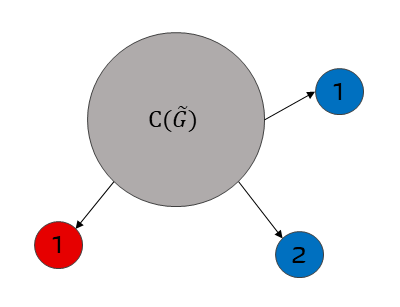
\includegraphics[width=2.5in]{Figures/condensation_digraph.png}
	\caption{Example of a network condensation digraph C(G). The people interactions are summarized as a single node, there are then one source of fake news (red) and two sources of real news (blue).}
	\label{pics:condensation_digraph_example}
\end{figure}
Figure~\ref{pics:condensation_digraph_example} shows an example condensation digraph for a network with irreducible $\tilde{A}$, one source of fake news and two sources of real news. The condensation is in general composed of $n_{Sources}+1$ nodes. The sources are all represented by sinks and the network of people by a single node connected to all sinks. \newline
All strongly connected components are furthermore acyclic: both the sources and the individuals have self-loops.
According to theorem 5.2 from the lecture notes, for a row-stochastic matrix A with multiple aperiodic sinks ($n_{Sources} \geq 2$), the following holds:
\begin{enumerate}
	\item
	A is semi-convergent.
	\item
	The eigenvalue 1 is semi-simple with multiplicity $n_{Sources}$ and all other eigenvalues $|\mu|<1$.
	\item
	The left eigenvectors $w^p \in \mathbb{R}^n$, $p\in \{1,...,n_{Sources}\}$, of A corresponding to the eigenvalue 1 can be selected to satisfy: $w^p\geq0,\ 1_n^Tw^p=1$, $w^p_i>0$ if and only if node i belongs to sink p.
	\item
	$
	x_{\infty}^i = 
	\begin{cases}
	(w^p)^Tx(0),& \text{node i $\in$ sink p}\\
	\sum_{p=1}^{n_{Sources}} z_{i,p}((w^p)^Tx(0)), & \text{otherwise}
	\end{cases}
	$
	where $z_{i,p},\ p\in\{1,...,n_{Sources}\}$, are convex combination coefficients and $z_{i,p} > 0$ if and only if there exists a directed path from node i to the sink p. This is always true for the individuals in this case making $z_{i,p} > 0\ \forall\ p \in \{1,...,n_{Sources}\}$ and $i \in \{1,...,n_{People}\}$.
\end{enumerate}
The third statement for the treated scenario implies $(w^p)^T = (0_{1 \times n_{People}},\ 0_{1 \times (p-1)},\ 1,\ 0_{1 \times (n_{Sources}-p)})$. This is because there is only one node in each sink p. The index referring to that node is therefore the only one different from zero in $w^p$. $1_n^Tw=1$ enforces its value to be exactly equal to 1. By plugging this result into iv), one can obtain the following:
$$
x_{\infty}^i = 
\begin{cases}
	x(0)^{n_{People}+p},& \text{node i $\in$ sink p}\\
	\sum_{p=1}^{n_{Sources}} z_{i,p}(x(0)^{n_{People}+p}), & \text{otherwise}
\end{cases}
$$
where $x(0)^{n_{People}+p}$ is the ($n_{People}+p$)th element of x(0). The steady state value of x therefore does not depend on the population initial conditions. It just depends on the sources'. Furthermore, it depends on $z_{i,p}$, whose value is strictly greater than zero for the population as  illustrated earlier. Their exact value depends on the random variables in our model and therefore cannot be estimated in general. (verificare) \newline
The result can be further simplified by plugging in the values of the initial conditions (-1 for fake and +1 for real news sources):
$$
x_{\infty}^i = 
\begin{cases}
\delta_p,& \text{node i $\in$ sink p}\\
\sum_{p=1}^{n_{Sources}} z_{i,p}\delta_p, & \text{otherwise}
\end{cases}
$$
where 
$
\delta_p = 
\begin{cases}
1,& \text{sink p is real news source}\\
-1,& \text{sink p is fake news source}
\end{cases}
$
$z_{i,p},\ p\in\{1,...,n_{Sources}\}$, are convex combination coefficients, which means that $\sum_{p=1}^{n_{Sources}} z_{i,p} = 1$ $\forall$ i.
If there is only one type of sources (either fake or real news), then $\sum_{p=1}^{n_{Sources}} z_{i,p}\delta = \delta*\sum_{p=1}^{n_{Sources}} z_{i,p} = \delta$ which is either +1 or -1 depending on whether the only type of source is real or fake: 
$x_\infty = 
\begin{cases}
1_n,& \text{Only real news sources}\\
-1_n,& \text{Only fake news sources}
\end{cases}$ 
\subsection{$n_{Sources} = 1$}
If $n_{Sources}=1$, then there is either a single fake or real news source. The condensation digraph contains a single aperiodic sink, which is composed by the source itself. The source is reachable from every node in G and the other nodes are reachable from every node in the graph but from the source. This makes the divulger the only globally reachable node in the graph. Its subgraph is furthermore aperiodic. From this it follows for the row-stochastic matrix A:
\begin{enumerate}
	\item
	The eigenvalue 1 is simple and all other eigenvalues $\mu$ satisfy $|\mu|<1$
	\item
	A is semi-convergent and $lim_{k->\infty} A^k = 1_n w^T$, where $w \in \mathbb{R}^n$ satisfies $w>=0, 1_n^T w = 1$, and $w^TA=w^T$
	\item
	$w>=0$ is the left dominant eigenvector of A and $w_i>0$ if and only if $i$ is globally reachable. As previously discussed, this is only the case for the single source in the treated example. \newline
	$\implies$ $w^T = (0,...,0,1)$.
	\item
	$x_\infty = (w^T x(0))1_n = x(0)^n 1_n = 	\begin{cases}
	1_n,& \text{Real news source}\\
	-1_n, & \text{Fake news source}
	\end{cases}$
	\newline The whole network would therefore converge to the source opinion for any people's initial conditions.
\end{enumerate}